\documentclass[]{article}
\usepackage{lmodern}
\usepackage{amssymb,amsmath}
\usepackage{ifxetex,ifluatex}
\usepackage{fixltx2e} % provides \textsubscript
\ifnum 0\ifxetex 1\fi\ifluatex 1\fi=0 % if pdftex
  \usepackage[T1]{fontenc}
  \usepackage[utf8]{inputenc}
\else % if luatex or xelatex
  \ifxetex
    \usepackage{mathspec}
  \else
    \usepackage{fontspec}
  \fi
  \defaultfontfeatures{Ligatures=TeX,Scale=MatchLowercase}
\fi
% use upquote if available, for straight quotes in verbatim environments
\IfFileExists{upquote.sty}{\usepackage{upquote}}{}
% use microtype if available
\IfFileExists{microtype.sty}{%
\usepackage{microtype}
\UseMicrotypeSet[protrusion]{basicmath} % disable protrusion for tt fonts
}{}
\usepackage[margin=2cm]{geometry}
\usepackage{hyperref}
\hypersetup{unicode=true,
            pdftitle={Do RATs save lives?},
            pdfauthor={Richard Pilbery and M. Dawn Teare},
            pdfborder={0 0 0},
            breaklinks=true}
\urlstyle{same}  % don't use monospace font for urls
\usepackage{natbib}
\bibliographystyle{apalike}
\usepackage{longtable,booktabs}
\usepackage{graphicx,grffile}
\makeatletter
\def\maxwidth{\ifdim\Gin@nat@width>\linewidth\linewidth\else\Gin@nat@width\fi}
\def\maxheight{\ifdim\Gin@nat@height>\textheight\textheight\else\Gin@nat@height\fi}
\makeatother
% Scale images if necessary, so that they will not overflow the page
% margins by default, and it is still possible to overwrite the defaults
% using explicit options in \includegraphics[width, height, ...]{}
\setkeys{Gin}{width=\maxwidth,height=\maxheight,keepaspectratio}
\IfFileExists{parskip.sty}{%
\usepackage{parskip}
}{% else
\setlength{\parindent}{0pt}
\setlength{\parskip}{6pt plus 2pt minus 1pt}
}
\setlength{\emergencystretch}{3em}  % prevent overfull lines
\providecommand{\tightlist}{%
  \setlength{\itemsep}{0pt}\setlength{\parskip}{0pt}}
\setcounter{secnumdepth}{5}
% Redefines (sub)paragraphs to behave more like sections
\ifx\paragraph\undefined\else
\let\oldparagraph\paragraph
\renewcommand{\paragraph}[1]{\oldparagraph{#1}\mbox{}}
\fi
\ifx\subparagraph\undefined\else
\let\oldsubparagraph\subparagraph
\renewcommand{\subparagraph}[1]{\oldsubparagraph{#1}\mbox{}}
\fi

%%% Use protect on footnotes to avoid problems with footnotes in titles
\let\rmarkdownfootnote\footnote%
\def\footnote{\protect\rmarkdownfootnote}

%%% Change title format to be more compact
\usepackage{titling}

% Create subtitle command for use in maketitle
\newcommand{\subtitle}[1]{
  \posttitle{
    \begin{center}\large#1\end{center}
    }
}

\setlength{\droptitle}{-2em}
  \title{Do RATs save lives?}
  \pretitle{\vspace{\droptitle}\centering\huge}
  \posttitle{\par}
  \author{Richard Pilbery and M. Dawn Teare}
  \preauthor{\centering\large\emph}
  \postauthor{\par}
  \predate{\centering\large\emph}
  \postdate{\par}
  \date{2018-07-02}

\usepackage{booktabs}
\usepackage{amsthm}
\makeatletter
\def\thm@space@setup{%
  \thm@preskip=8pt plus 2pt minus 4pt
  \thm@postskip=\thm@preskip
}
\makeatother
\usepackage{booktabs}
\usepackage{longtable}
\usepackage{array}
\usepackage{multirow}
\usepackage[table]{xcolor}
\usepackage{wrapfig}
\usepackage{float}
\usepackage{colortbl}
\usepackage{pdflscape}
\usepackage{tabu}
\usepackage{threeparttable}
\usepackage[normalem]{ulem}

\AtBeginDocument{\let\maketitle\relax}

\usepackage{amsthm}
\newtheorem{theorem}{Theorem}[section]
\newtheorem{lemma}{Lemma}[section]
\theoremstyle{definition}
\newtheorem{definition}{Definition}[section]
\newtheorem{corollary}{Corollary}[section]
\newtheorem{proposition}{Proposition}[section]
\theoremstyle{definition}
\newtheorem{example}{Example}[section]
\theoremstyle{definition}
\newtheorem{exercise}{Exercise}[section]
\theoremstyle{remark}
\newtheorem*{remark}{Remark}
\newtheorem*{solution}{Solution}
\begin{document}
\maketitle

\hypertarget{do-rats-save-lives-a-retrospective-analysis-of-out-of-hospital-cardiac-arrest-in-an-english-ambulance-service}{%
\section{Do RATs save lives? A retrospective analysis of out-of-hospital
cardiac arrest in an English Ambulance
Service}\label{do-rats-save-lives-a-retrospective-analysis-of-out-of-hospital-cardiac-arrest-in-an-english-ambulance-service}}

\hypertarget{author-information}{%
\subsection{Author information}\label{author-information}}

\textbf{Richard Pilbery}\\
Research paramedic\\
Yorkshire Ambulance Service NHS Trust\\
Springhill, Brindley Way\\
Wakefield 41 Business Park\\
Wakefield\\
WF2 0XQ

ORCID: \url{https://orcid.org/0000-0002-5797-9788}

email: \href{mailto:r.pilbery@nhs.net}{\nolinkurl{r.pilbery@nhs.net}}\\
tel:

\textbf{Dr.~M. Dawn Teare}\\
Reader in Epidemiology and Biostatistics\\
University of Sheffield

\textbf{Word count:} 2721

\textbf{Keywords:} Out-of-hospital, cardiac arrest, paramedic

\hypertarget{abstract}{%
\subsection{Abstract}\label{abstract}}

\hypertarget{introduction}{%
\subsubsection{Introduction}\label{introduction}}

Out of hospital cardiac arrest (OHCA) is a major public health problem
leading to a substantial number of deaths in the UK. Survival to
discharge rates in the UK have remained below that of the best
performing European countries. In response to this, Yorkshire Ambulance
Service (YAS) has introduced several initiatives to improve outcome from
OHCA including the introduction of Red Arrest Teams (RATs).

This study aims to determine the impact of the RATs on survival to 30
days and return of spontaneous circulation (ROSC) at hospital.

\hypertarget{methods}{%
\subsubsection{Methods}\label{methods}}

A retrospective cohort study analysing routinely collected data was
undertaken. All adult (≥18 years) OHCAs entered onto the YAS computer
aided dispatch (CAD) system between the 1st October, 2015 and 30th
September, 2017 were included if the patient was resuscitated, and the
cause of the arrest was considered to be medical in origin.
Multivariable logistic regression models were created to enable
adjustment for common predictors of survival and ROSC.

\hypertarget{results}{%
\subsubsection{Results}\label{results}}

\textbf{ENTER RESULTS HERE}

\hypertarget{conclusion}{%
\subsubsection{Conclusion}\label{conclusion}}

The presence of a RAT paramedic was associated with a small increase in
survival to 30 days and ROSC on arrival at hospital, although neither
were statistically significant. Larger prospective studies are required
to determine the effect of roles such as RAT on outcomes from OHCA

\hypertarget{intro}{%
\section{Introduction}\label{intro}}

Out of hospital cardiac arrest (OHCA) is a major public health problem
leading to a substantial number of deaths in Europe. Since routine
reporting of cardiac arrest outcomes commenced in the United Kingdom in
2011, it is evident that even in the Utstein group of patients
(i.e.~those who suffered a witnessed cardiac arrest of presumed cardiac
cause, were resuscitated, and found to be in a shockable rhythm on
arrival of the ambulance service), survival to discharge rates have
remained under 30\%, well below that of the best performing European
countries \citep{grasner_eureca_2016}.

In response to this, Yorkshire Ambulance Service (YAS) has introduced
several initiatives to improve outcome from OHCA including:

\begin{itemize}
\tightlist
\item
  Teaching members of the public, particularly school-age children,
  Basic Life Support (BLS)
\item
  Improving telephone triage of 999 calls to ensure that there is a
  minimum delay in recognition of cardiac arrest and commencement of
  telephone CPR
\item
  Introducing Red Arrest Teams across Yorkshire.
\end{itemize}

The Red Arrest Teams (RATs) consist of operational managers who attend a
three-day training course, focusing on the technical and non-technical
skills that are required to effectively team lead an OHCA and provide
high quality post-resuscitation care. RATs have been deployed throughout
Yorkshire, ensuring that all members of the public can benefit from the
initiative, and not just one locality. The RAT scheme is also different
from some other Services, such as those provided by London and South
East Coast ambulance services, in that the training is not at Masters
degree level or associated with a prolonged training period, making it
inexpensive and pragmatic to run despite high operational pressures and
economic constraints.

Following the introduction of the RAT scheme and other initiatives, YAS
achieved Utstein survival to discharge rates in excess of 41\%, compared
to the national average in the same period of 28\%, in 2015--2016.
However, the relative contribution of each aspect of the initiatives
that have been introduced within the Service is unknown.

This study aims to determine the impact of the RATs on outcomes from
OHCA. The primary outcome is a comparison of survival to discharge from
hospital, between groups of patients where a RAT was present, compared
to those with no RAT attendance. The secondary outcome is a comparison
of return of spontaneous circulation (ROSC) at hospital between the same
groups as the primary outcome.

\hypertarget{methods-1}{%
\section{Methods}\label{methods-1}}

A retrospective cohort study analysing routinely collected data between
October 2015 and September 2017 was undertaken, to compare differences
in outcome from out-of-hospital cardiac arrests, between incidents where
a RAT paramedic was present and incidents where a RAT paramedics was not
present. Multiple logistic regression was used to adjust for factors
that are known to affect outcome from OHCA, and the primary outcome was
survival to 30 days.

\hypertarget{setting}{%
\subsection{Setting}\label{setting}}

Yorkshire Ambulance Service NHS Trust (YAS) provides 24-hour emergency
and healthcare services for the county of Yorkshire, in England. The
county has a population of approximately five million, spread over
almost 6,000 square miles of varied terrain, including isolated moors
and dales, coastline and urban areas. YAS operates 62 ambulance
stations, and in 2016--17, received 895,700 emergency calls which
resulted in 723,935 attendances by YAS staff.

\hypertarget{red-arrest-team}{%
\subsection{Red Arrest Team}\label{red-arrest-team}}

The Red Arrest Team (RAT) concept in YAS started thanks to staff in the
Hull area taking the initiative and undertaking the role informally in
2013. The following year, based on part on the work of 3RU in Scotland
\citep{clarke_specialist_2014} and an American Heart Association
consensus statement on CPR quality and improving outcomes from cardiac
arrest \citep{meaney_cardiopulmonary_2013}, formal pilots were conducted
in Bradford, Doncaster, Harrogate, Hull, Leeds and York. RAT members
were provided with a 1-day training course, with a syllabus focused on
team-leadership and other non-technical skills, in addition to doing the
basics well (e.g.~increasing chest compression fraction, providing
high-quality ventilation). Following the pilot phase, a widespread
roll-out occured from October 2015 to all existing operational line
managers (referred to locally as clinical supervisors). From 2016/17,
the RAT course was extended to 3 days, to include additional skills such
as post-ROSC care, and included an assessment of competence.

YAS has a pre-determined respsonse to cardiac arrest calls which is
compromised of at least two resources; including a conveying resource
i.e.~an ambulance, and at least one Advanced Life Support (ALS) provider
(paramedic). A RAT paramedic is also dispatched if they are available,
and are located less than 20 minutes drive from the patient's location.

\hypertarget{data-collection}{%
\subsection{Data collection}\label{data-collection}}

Cardiac arrests were identified from the YAS computer aided dispatch
(CAD) system via a bespoke database query, and by review of patient care
records by a research paramedic. Outcome data was obtained from the YAS
clinical audit and business intelligence units as part of their routine
reporting of ambulance quality indicators
\citep{nhs_england_ambulance_2015}. The clinical directorate at YAS
provided a list of RAT-trained paramedics, along with the date they
completed their training, in addition to the callsigns of RAT vehicles.
This was cross-referenced against the ambulance staff who had attended a
cardiac arrest, to determine if a RAT had attended the incident. When
calculating the elapsed time from cardiac arrest to RAT arrival, only
the first RAT-trained paramedic's time was included (i.e.~if more than
one RAT-trained paramedic was in attendance, subsequent RAT arrival
times were ignored). Where the cardiac arrest onset time was not known,
the time of the emergency call time was used instead.

In addition to the RAT presence and time of arrival, the age, gender and
location of the patient was recorded. Other variables included whether
bystander CPR occured, whether the OHCA was witnessed, and if so, by
whom, the response time of the first YAS response, the presenting
rhythm, the prehospital outcome (i.e.~whether the patient was
transported to hospital or had a Recognition of Life Extinct, ROLE
performed on scene) and the hospital outcome, consisting of the presence
of ROSC at hospital, and the survival outcome.

\hypertarget{participants}{%
\subsection{Participants}\label{participants}}

All adult (18 years and over) OHCAs entered onto the YAS CAD system
between 00:00:00 on the 1st October, 2015 and 23:59:59 on the 30th
September, 2017 were included if the patient was resuscitated, and the
cause of the arrest was considered to be medical in origin. Incidents
were exlcuded if the patient care record could not be located,
resuscitation was not commenced or continued by a member of YAS staff,
or the cardiac arrest was of traumatic origin or occured in-hospital. In
addition, in an attempt to account for appropriate termination of futile
resuscitations, that form part of the RAT role, all cardiac arrests
where resuscitation was terminated within 10 minutes of RAT arrival on
scene, or 10 minutes of the first crew arrival time on scene, were
excluded.

\hypertarget{statistical-analysis}{%
\subsection{Statistical analysis}\label{statistical-analysis}}

Multivariable logistic regression models were created using the
statistics package, R \citep{R-base}, to enable adjustment for known
factors that affect OHCA survival and ROSC, including patient age,
gender, location, whether the arrest was witnessed and if so, by whom
(bystander or ambulance crew), whether bystander CPR was performed,
response time and first monitored cardiac rhythm. In addition, the
presence or absence of a RAT paramedic was noted.

\hypertarget{ethics}{%
\subsection{Ethics}\label{ethics}}

Research Ethics Committee approval was not required as this study was
classed as a service evaluation.

\hypertarget{results-1}{%
\section{Results}\label{results-1}}

\begin{table}

\caption{\label{tab:demotable}Demographic details of cardiac arrests}
\centering
\begin{tabular}[t]{llll}
\toprule
Variable & RAT & No RAT & All\\
\midrule
n (\%) & 2000 (34.1) & 3868 (65.9) & 5868 (100)\\
Median age (IQR) years & 70 (57--80) & 72 (60--82) & 71 (59--81)\\
Male n (\%) & 1256 (62.8) & 2420 (62.6) & 3676 (62.6)\\
Bystander CPR n (\%) & 1344 (67.2) & 2366 (61.2) & 3710 (63.2)\\
Median response time by crew mins (IQR) & 7 (5--10) & 7 (4--10) & 7 (4--10)\\
Median response time by RAT mins (IQR) & 15 (10--22) & NA (NA--NA) & 15 (10--21)\\
\addlinespace[0.3em]
\multicolumn{4}{l}{\textbf{Witness status n (\%)}}\\
\hspace{1em}Unwitnessed arrests & 806 (40.3) & 1433 (37) & 2239 (38.2)\\
\hspace{1em}Witnessed arrests & 1194 (59.7) & 2435 (63) & 3629 (61.8)\\
\hspace{1em}Witnessed arrest by EMS & 129 (6.5) & 565 (14.6) & 694 (11.8)\\
\hspace{1em}Witnessed arrest by bystander & 1065 (53.2) & 1870 (48.3) & 2935 (50)\\
\addlinespace[0.3em]
\multicolumn{4}{l}{\textbf{Presenting rhythm n (\%)}}\\
\hspace{1em}Shockable & 515 (25.8) & 997 (25.8) & 1512 (25.8)\\
\hspace{1em}PEA & 402 (20.1) & 863 (22.3) & 1265 (21.6)\\
\hspace{1em}Asystole & 1083 (54.1) & 2008 (51.9) & 3091 (52.7)\\
\addlinespace[0.3em]
\multicolumn{4}{l}{\textbf{Location n (\%)}}\\
\hspace{1em}Private & 1500 (75) & 2822 (73) & 4322 (73.7)\\
\hspace{1em}Public & 329 (16.4) & 570 (14.7) & 899 (15.3)\\
\hspace{1em}Nursing home & 162 (8.1) & 357 (9.2) & 519 (8.8)\\
\hspace{1em}Ambulance & 9 (0.4) & 119 (3.1) & 128 (2.2)\\
\addlinespace[0.3em]
\multicolumn{4}{l}{\textbf{Prehospital measure n (\%)}}\\
\hspace{1em}ROLE after >10 mins resus & 917 (45.9) & 2098 (54.2) & 3015 (51.4)\\
\hspace{1em}ROLE after <10 mins resus & 169 (8.5) & 26 (0.7) & 195 (3.3)\\
\hspace{1em}Transported to hospital & 914 (45.7) & 1744 (45.1) & 2658 (45.3)\\
\addlinespace[0.3em]
\multicolumn{4}{l}{\textbf{Hospital/Survival measures n (\%)}}\\
\hspace{1em}ROSC at hospital & 532 (26.6) & 1054 (27.2) & 1586 (27)\\
\hspace{1em}Survived & 132 (6.6) & 284 (7.3) & 416 (7.1)\\
\hspace{1em}Survival status unknown & 178 (8.9) & 387 (10) & 565 (9.6)\\
\hspace{1em}Died in hospital & 604 (30.2) & 1073 (27.7) & 1677 (28.6)\\
\bottomrule
\multicolumn{4}{l}{\textbf{Note: } }\\
\multicolumn{4}{l}{NA: Not applicable}\\
\end{tabular}
\end{table}

\begin{figure}
\centering
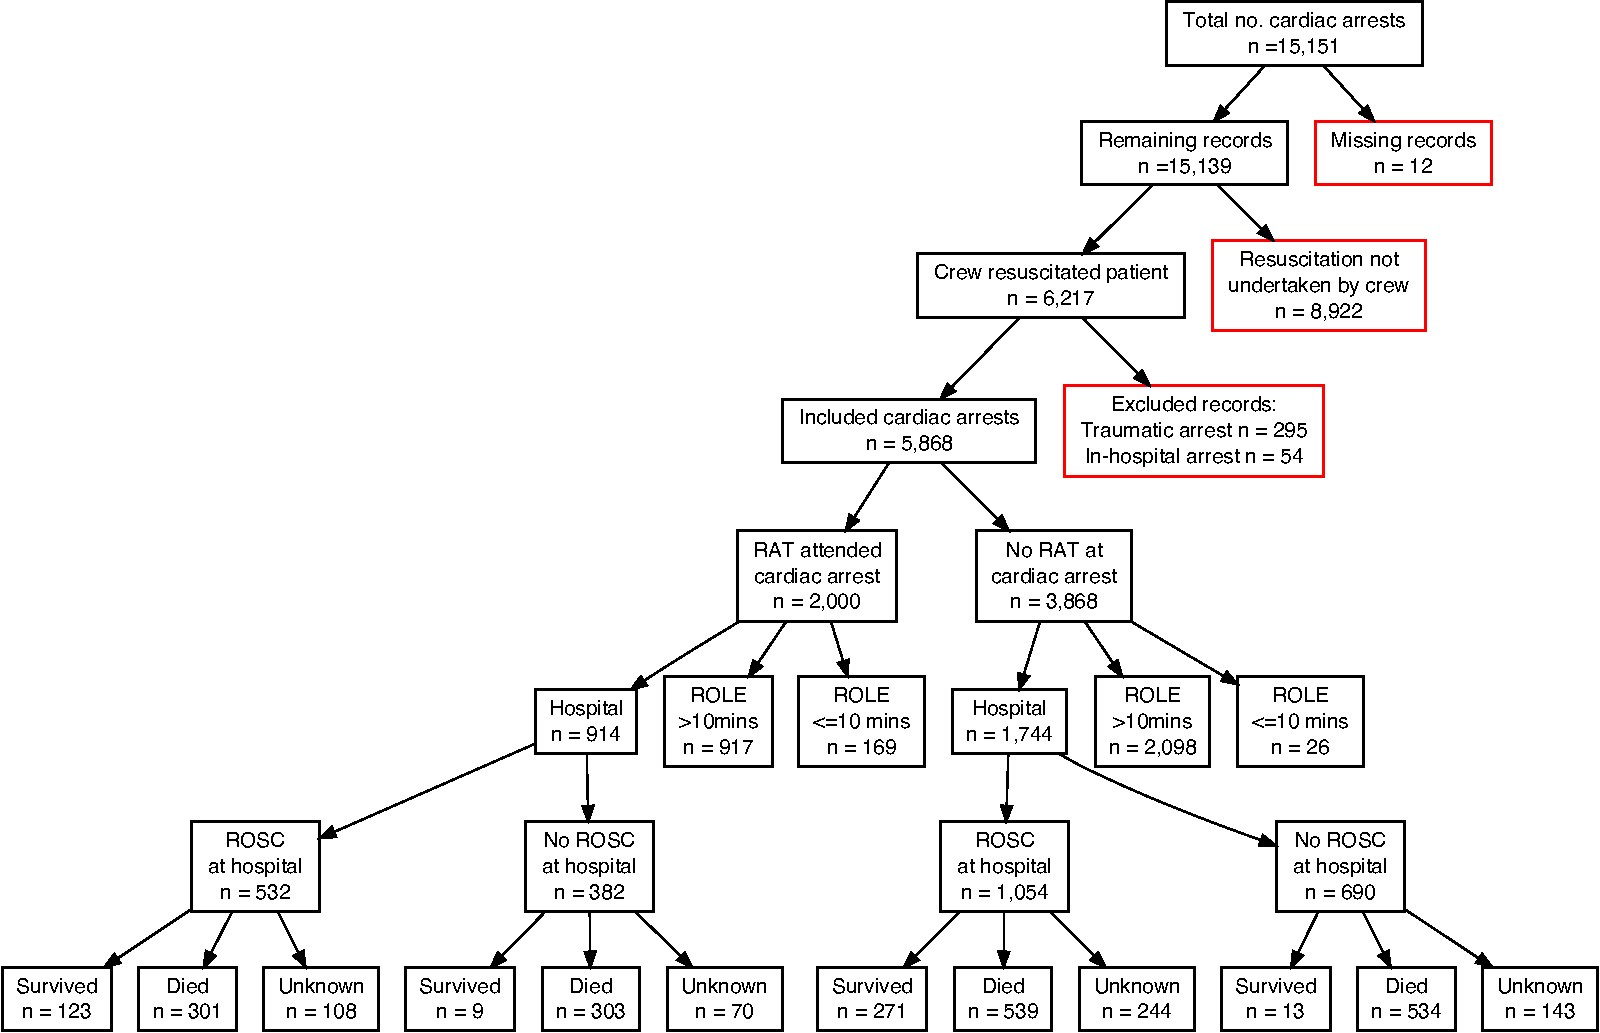
\includegraphics{RAT-evaluation_files/figure-latex/figure1-1.pdf}
\caption{\label{fig:figure1}Patients suffering an OHCA in the study period}
\end{figure}

Between the 1st October, 2015 and 30th September, 2017, there were
15,151 cardiac arrests that were attended by Yorkshire Ambulance
Service. After removing 12 cases where no PCR could be located, 15,139
remained. There were 8,922 patients who had no resuscitated attempted by
YAS ambulance personnel, and 6,217 cardiac arrests where resuscitation
was attempted. Another 349 were removed since the cardiac arrest was
either of traumatic origin (295 incidents), or was an in-hospital
cardiac arrest (54 incidents). This resulted in 5,868 cardiac arrests
suitable for inclusion in this evaluation (Figure \ref{fig:figure1}).

During the 2-year data collection period, 123/158 (77.8\%) RATs attended
2,000/5,868 (34.1\%) incidents, with each RAT attending a median of 13
cardiac arrests (IQR 7--23, minimum 1, maximum 78). The demographics of
the two patient groups (RAT/non-RAT) were similar (Table
\ref{tab:demotable}), although there were several significant
differences in the distribution of patient demographic and OHCA factors
between the RAT attended and non-RAT attended OHCAs.

RATs attended OHCAs with slightly younger patients (median 70 years vs
72 years), a higher proportion of bystander-witnessed arrests (53.2\% vs
48.3\%) and were more likely to terminate an OHCA within 10 minutes of
arriving on scene (8.5 vs 0.7). Conversely, in the non-RAT OHCA group,
there was a significantly higher proportion of witnessed arrests by a
member of the ambulance service (14.6\% vs 6.5\%), and cardiac arrests
that occurred in an ambulance (3.1\% vs 0.4\%).

There were 2,658 patients who were conveyed to hospital, although the
survival outcome for 605 incidents was intially unknown. Clinical audit
had not identified 519 incidents, and a further 86 OHCAs that had been
identified by clinical audit, received no survival outcome data from the
destination hospital. However, as a result of screening of the CAD and
review of PRFs, the outcome of a further 40 was determined, although
none of these patients survived to discharge. This resulted in a final
total of 565/2,658 (21.3\%) patients with no surival outcome status.

\hypertarget{roll-out-of-the-rat-scheme}{%
\subsection{Roll-out of the RAT
scheme}\label{roll-out-of-the-rat-scheme}}

The RAT scheme was rolled out across the region over the course of the
service evaluation, with coverage expanding from the pilot sites. The
proportion of cardiac arrests attended during the data collection period
is shown in Figure \ref{fig:ratrollout}.

\begin{figure}
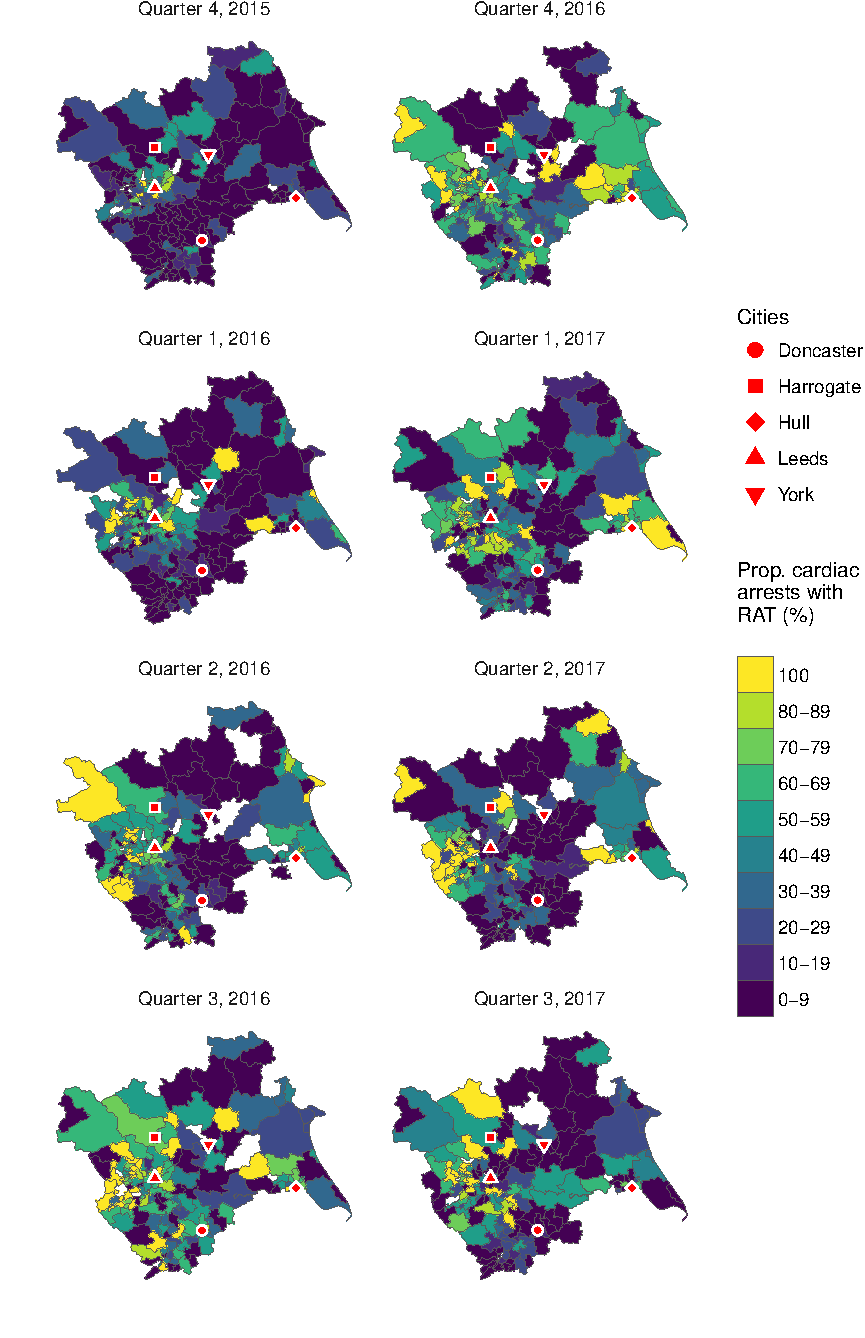
\includegraphics{RAT-evaluation_files/figure-latex/ratrollout-1} \caption{Proportion of cardiac arrests attended by a RAT, stratified by yearly quarter}\label{fig:ratrollout}
\end{figure}

\rowcolors{2}{gray!6}{white}
\begin{table}

\caption{\label{tab:model1}Results of regression modelling of survival to discharge}
\centering
\begin{tabular}[t]{>{\raggedright\arraybackslash}p{4cm}lll}
\hiderowcolors
\toprule
Variable & OR & 95\% CI & p-value\\
\midrule
\showrowcolors
Age & 0.96 & 0.95--0.97 & 0.00\\
Male gender & 1.37 & 0.99--1.9 & 0.06\\
Bystander CPR & 0.94 & 0.65--1.37 & 0.76\\
Arrest to Crew arrival time (per elapsed minute) & 1 & 0.98--1.01 & 0.62\\
\addlinespace[0.3em]
\multicolumn{4}{l}{\textbf{Witness status}}\\
\hspace{1em}Unwitnessed & Reference & Reference & Reference\\
\hspace{1em}Witnessed: bystander & 1.78 & 1.18--2.71 & 0.01\\
\hspace{1em}Witnessed: EMS & 4.98 & 2.55--9.85 & 0.00\\
\addlinespace[0.3em]
\multicolumn{4}{l}{\textbf{Presenting rhythm}}\\
\hspace{1em}Asystole & Reference & Reference & Reference\\
\hspace{1em}PEA & 0.95 & 0.55--1.63 & 0.85\\
\hspace{1em}Shockable & 10.11 & 6.8--15.39 & 0.00\\
\addlinespace[0.3em]
\multicolumn{4}{l}{\textbf{Location}}\\
\hspace{1em}Private & Reference & Reference & Reference\\
\hspace{1em}Public & 2.07 & 1.48--2.88 & 0.00\\
\hspace{1em}Nursing home & 0.41 & 0.11--1.14 & 0.12\\
\hspace{1em}Ambulance & 2.07 & 0.93--4.75 & 0.08\\
\addlinespace[0.3em]
\multicolumn{4}{l}{\textbf{Status at ED}}\\
\hspace{1em}ROSC at hospital & 54.82 & 35.46--89.12 & 0.00\\
\addlinespace[0.3em]
\multicolumn{4}{l}{\textbf{RAT}}\\
\hspace{1em}No RAT present & Reference & Reference & Reference\\
\hspace{1em}RAT present & 1.01 & 0.74--1.38 & 0.93\\
\hspace{1em}Unadjusted OR & 0.98 & 0.79--1.21 & 0.84\\
\bottomrule
\multicolumn{4}{l}{\textbf{Note: } }\\
\multicolumn{4}{l}{NA: Not applicable}\\
\end{tabular}
\end{table}
\rowcolors{2}{white}{white}

\rowcolors{2}{gray!6}{white}
\begin{table}

\caption{\label{tab:model2}Results of regression modelling of ROSC on arrival at hospital}
\centering
\begin{tabular}[t]{>{\raggedright\arraybackslash}p{4cm}lll}
\hiderowcolors
\toprule
Variable & OR & 95\% CI & p-value\\
\midrule
\showrowcolors
Age & 0.99 & 0.99--0.99 & 0.00\\
Male gender & 0.83 & 0.72--0.94 & 0.01\\
Bystander CPR & 1 & 0.86--1.16 & 0.95\\
Arrest to Crew arrival time (per elapsed minute) & 0.99 & 0.98--1 & 0.03\\
\addlinespace[0.3em]
\multicolumn{4}{l}{\textbf{Witness status}}\\
\hspace{1em}Unwitnessed & Reference & Reference & Reference\\
\hspace{1em}Witnessed: bystander & 1.72 & 1.48--2 & 0.00\\
\hspace{1em}Witnessed: EMS & 1.88 & 1.38--2.55 & 0.00\\
\addlinespace[0.3em]
\multicolumn{4}{l}{\textbf{Presenting rhythm}}\\
\hspace{1em}Asystole & Reference & Reference & Reference\\
\hspace{1em}PEA & 1.69 & 1.42--2 & 0.00\\
\hspace{1em}Shockable & 4.34 & 3.72--5.08 & 0.00\\
\addlinespace[0.3em]
\multicolumn{4}{l}{\textbf{Location}}\\
\hspace{1em}Private & Reference & Reference & Reference\\
\hspace{1em}Public & 1.16 & 0.98--1.38 & 0.08\\
\hspace{1em}Nursing home & 0.96 & 0.74--1.23 & 0.74\\
\hspace{1em}Ambulance & 1.18 & 0.76--1.82 & 0.46\\
\addlinespace[0.3em]
\multicolumn{4}{l}{\textbf{RAT}}\\
\hspace{1em}No RAT present & Reference & Reference & Reference\\
\hspace{1em}RAT present & 1.13 & 0.99--1.29 & 0.08\\
\hspace{1em}Unadjusted OR & 1.09 & 0.97--1.24 & 0.16\\
\bottomrule
\multicolumn{4}{l}{\textbf{Note: } }\\
\multicolumn{4}{l}{NA: Not applicable}\\
\end{tabular}
\end{table}
\rowcolors{2}{white}{white}

\hypertarget{regression-models}{%
\subsection{Regression models}\label{regression-models}}

The outcome of the regression models for survival to discharge and ROSC
on arrival at hospital, can be seen in Tables \ref{tab:model1} and
\ref{tab:model2}. These results suggest that a RAT on scene is
associated with a slight increase in the odds of survival to 30 days (OR
1.01, 95\%CI 0.74--1.38) and odds of ROSC on arrival at hospital (OR
1.13, 95\%CI 0.99--1.29), compared to the odds of not having a RAT
present, although neither of these results are statistically
significant.

\hypertarget{discussion}{%
\section{Discussion}\label{discussion}}

The unadjusted odds ratios suggest that there is no significant increase
in the odds of survival to discharge or ROSC at hospital when a RAT is
present, compared to OHCAs where no RAT is present (OR 0.98, 95\%CI
0.79--1.21 and OR 1.09, 95\%CI 0.97--1.24 respectively). When adjusting
for factors that are known to affect outcome from OHCA using multiple
logistic regression, the results from this study indicate that there is
an slight increase in the odds of survival to 30 days when a RAT is
present (OR 1.01, 95\%CI 0.74--1.38, p=0.93), and in the odds of ROSC at
hospital, compared to OHCA without a RAT present (OR 1.13, 95\%CI
0.99--1.29, p=0.08), although both results are not statistically
significant.

Drawing firm conclusions about the primary outcome in this study has
been impaired by the high level of missing survival outcome data
(565/2658, 21.3\% of outcomes are missing from the subset of patients
who were taken to hospital). In addition, there were some significant
differences in the distribution of patient demographic and OHCA factors
between the RAT attended and non-RAT attended OHCAs. RAT attended OHCAs
had younger patients and a higher proportion of bystander witnessed
arrests. Conversely, in the non-RAT OHCA group, there was a
significantly higher proportion of witnessed arrests by a member of the
ambulance service and cardiac arrests that occured in an ambulance
(Table \ref{tab:demotable}).

It appears from Figure \ref{fig:ratrollout} that there was temporal and
spatial variation of the proportion of OHCAs attended by a RAT. The
scheme rolled out from the pilot sites in October 2015 onwards, and
appeared to reach a peak in Quarter 3 and 4 of 2016. However, the
proportion of arrests attended by the RAT declined in 2017. It is
possible that this was due to operational presssures resulting in the
inappropriate tasking of RAT resources from OHCAs to other emergency
calls that could not be covered.

\hypertarget{comparison-with-other-systems}{%
\subsection{Comparison with other
systems}\label{comparison-with-other-systems}}

Making comparisons with the literature is difficult, given that there is
limited robust data from other pre-hospital emergency care teams and
their affect on survival outcomes. Most published studies compare
physician-based critical care teams to advanced life support (ALS)
paramedics. A recent systematic review found scant evidence that these
teams offer a survival benefit in OHCA
\citep{von_vopelius-feldt_systematic_2017}, with three of the six papers
included in the review finding no benefit in OHCA outcomes. However, as
the authors of the review point out, study design, team tasking and
type-2 errors all effect the findings of included studies. It is
possible that these teams are of greatest benefit post-ROSC or during
protracted resuscitation, if they cannot be dispatched immediately.

There are few paramedic-only studies in the UK examining the use of
specialist teams to improve outcome from OHCA. The scheme that has
inspired at least two others in England, is the Resuscitation Rapid
Response Unit (3RU) in Scotland. Originally based in Edinburgh, it has
now expanded into all urban conurbations. However, the scheme has only
published results from early service evaluations, which demonstrated a
ROSC rate of 38\% in the Edinburg area in 2010/11, compared to a
national mean of 19.2\% at the time \citep{clegg_using_2012}.

Paramedics forming the 3RU, were volunteers who received advanced life
support-style training in addition to non-technical skills
\citep{clarke_specialist_2014}. However, since the scheme expanded, all
training is conducted through paid study leave and staff rostered onto
the unit \citep{short_3ru_2018}.

In North East Ambulance Service NHS Trust (NEAS), The cardiac arrest
response unit (CARU) was set up in 2014 to improve OHCA outcomes. As
with the RAT scheme in YAS, it was based on the work of 3RU. The group
was compromised of 11 senior paramedics who provided the majority of
coverage, although 11 of the cardiac arrests reported by
\citet{mcclelland_service_2016} were attended by a pre-hospital
emergency medicine (PHEM) doctor who was also a member of the team.
Coverage was limited to a single locality focussed around
Newcastle-Upon-Tyne and working hours of 07:00--17:00. Paramedics
forming part of the team completed the pre-hospital emergncey
resuscitation (SPHERe) course run by Promethes Medical Ltd.~and a
pre-hospital anaesthesics course run by the Great North Air Ambulance.
Maintenance of skills, was achieved by weekely training session
compromised of LAS drills and scenarios, although most of these were
voluntary and attended in the team's own time.

During its first year of operation, CARU was activated 333 times, and
attended 164 OHCAs. Compared to the rest of NEAS, CARU had a significant
increase in survival to discharge and ROSC on arrival at hospital
(unadjusted odds ratios of 2.08, 95\%CI 1.12--3.84 and 1.74, 95\%CI
1.19--2.54) \citep{mcclelland_service_2016}.

In London Ambulance Service (LAS), the role of the Advanced Paramedic
Practitioner (APP) was created in 2014, and attendance at OHCA is part
of the role. The only data published on their performance is from the
LAS cardiac arrest report, which shows an increase in ROSC at hospital
and survival to discharge figures compared to incidents where no APP was
in attendance (34.6\% and 12.1\%, versus 29.4\% and 9.5\%). However, as
with the previous data, these are unadjusted figures and the report
notes that VF/VT was the presenting rhythm in 30.2\% of cases attended
by an APP compared to 22.0\% in other LAS OHCAs
\citep{london_ambulance_service_nhs_trust_cardiac_2017}.

\hypertarget{limitations}{%
\subsection{Limitations}\label{limitations}}

This study is observational and retrospective, utilising routine data.
As such, causal links cannot be made. In addition, there is a
significant proportion of data missing form the primary outcome measure,
and the primary outcome is not as patient-centred as survival to
discharge with a favourable neurological outcome, for example. However,
neurological status of the patient at time of discharge (or to 30 days)
is not currently collected as part of the quality indicators for
ambulance services. To address issues with data reliability, the Trust
is embarking on a roll-out of electronic patient care records, which
should improve the reliability of data capture, although will not
guarantee that outcome data will always be provided by receiving
hospitals.

No adjustment was made for the receiving hospital in this analysis,
which may impact on patient survival outcomes
\citep{stub_hospital_2011, stub_hospital_2015}. In addition, only a
crude adjustment was made in an attempt to account for the RAT's
alternate role of ceasing futile resuscitation attempts, which may have
adversely affected the apparent survival benefit of a RAT presence.

\hypertarget{conclusion-1}{%
\section{Conclusion}\label{conclusion-1}}

In this study, the presence of a RAT paramedic was associated with a
small increase in survival to 30 days (OR 1.01, p=0.93) and ROSC on
arrival at hospital (OR 1.13, p=0.08), although neither were
statistically significant. The magnitude of missing survival outcomes
limits confidence in this robustness of this result. Further research
into the affect of roles such as RAT, particularly in schemes lead by
paramedics, is required.

\hypertarget{appendix-a}{%
\section{Appendix A}\label{appendix-a}}

\hypertarget{sensitivity-analysis}{%
\subsection{Sensitivity analysis}\label{sensitivity-analysis}}

These regression models only contain variables found to be statistically
significant in terms of contributing to the regression model. For
survival to 30 days, male gender, bystander CPR and arrest to crew
arrival time have been omitted, and for ROSC on arrival at hospital,
bystanderCPR and location have been removed from the model.

\rowcolors{2}{gray!6}{white}
\begin{table}

\caption{\label{tab:appendixaSURV}Results of regression modelling of survival to discharge}
\centering
\begin{tabular}[t]{>{\raggedright\arraybackslash}p{4cm}lll}
\hiderowcolors
\toprule
Variable & OR & 95\% CI & p-value\\
\midrule
\showrowcolors
Age & 0.96 & 0.95--0.97 & 0.00\\
\addlinespace[0.3em]
\multicolumn{4}{l}{\textbf{Witness status}}\\
\hspace{1em}Unwitnessed & Reference & Reference & Reference\\
\hspace{1em}Witnessed: bystander & 1.73 & 1.15--2.63 & 0.01\\
\hspace{1em}Witnessed: EMS & 5.54 & 3.31--9.39 & 0.00\\
\addlinespace[0.3em]
\multicolumn{4}{l}{\textbf{Presenting rhythm}}\\
\hspace{1em}Asystole & Reference & Reference & Reference\\
\hspace{1em}PEA & 0.99 & 0.57--1.7 & 0.98\\
\hspace{1em}Shockable & 10.74 & 7.26--16.27 & 0.00\\
\addlinespace[0.3em]
\multicolumn{4}{l}{\textbf{Location}}\\
\hspace{1em}Private & Reference & Reference & Reference\\
\hspace{1em}Public & 2.15 & 1.55--2.98 & 0.00\\
\hspace{1em}Nursing home & 0.39 & 0.11--1.08 & 0.10\\
\hspace{1em}Ambulance & 2.21 & 1.03--4.84 & 0.04\\
\addlinespace[0.3em]
\multicolumn{4}{l}{\textbf{Status at ED}}\\
\hspace{1em}ROSC at hospital & 53.99 & 34.96--87.71 & 0.00\\
\addlinespace[0.3em]
\multicolumn{4}{l}{\textbf{RAT}}\\
\hspace{1em}No RAT present & Reference & Reference & Reference\\
\hspace{1em}RAT present & 1.01 & 0.74--1.37 & 0.97\\
\bottomrule
\multicolumn{4}{l}{\textbf{Note: } }\\
\multicolumn{4}{l}{NA: Not applicable}\\
\end{tabular}
\end{table}
\rowcolors{2}{white}{white}

\rowcolors{2}{gray!6}{white}
\begin{table}

\caption{\label{tab:appendixaROSC}Results of regression modelling of ROSC on arrival at hospital}
\centering
\begin{tabular}[t]{>{\raggedright\arraybackslash}p{4cm}lll}
\hiderowcolors
\toprule
Variable & OR & 95\% CI & p-value\\
\midrule
\showrowcolors
Age & 0.99 & 0.99--0.99 & 0.00\\
Male gender & 0.84 & 0.73--0.96 & 0.01\\
Arrest to Crew arrival time (per elapsed minute) & 0.99 & 0.98--1 & 0.01\\
\addlinespace[0.3em]
\multicolumn{4}{l}{\textbf{Witness status}}\\
\hspace{1em}Unwitnessed & Reference & Reference & Reference\\
\hspace{1em}Witnessed: bystander & 1.74 & 1.5--2.02 & 0.00\\
\hspace{1em}Witnessed: EMS & 1.88 & 1.39--2.53 & 0.00\\
\addlinespace[0.3em]
\multicolumn{4}{l}{\textbf{Presenting rhythm}}\\
\hspace{1em}Asystole & Reference & Reference & Reference\\
\hspace{1em}PEA & 1.69 & 1.43--2 & 0.00\\
\hspace{1em}Shockable & 4.5 & 3.86--5.24 & 0.00\\
\addlinespace[0.3em]
\multicolumn{4}{l}{\textbf{RAT}}\\
\hspace{1em}No RAT present & Reference & Reference & Reference\\
\hspace{1em}RAT present & 1.13 & 0.99--1.29 & 0.08\\
\bottomrule
\multicolumn{4}{l}{\textbf{Note: } }\\
\multicolumn{4}{l}{NA: Not applicable}\\
\end{tabular}
\end{table}
\rowcolors{2}{white}{white}

\bibliography{RAT-EVAL.bib,packages.bib}


\end{document}
